\chapter{Question-Asking and Plan Inference}
\label{ch:question_plan}
\textbf{Salena Ashton, Stephen Kim, Loren Rieffer-Champlin, Liang Zhang,
Adarsh Pyarelal, Clayton Morrison}

\section{Introduction}

In the SAR scenario for ASIST's Minecraft virtual environment, teams of human players engage in cooperative behavior to search for, stabilize, and rescue victims within a collapsed building. As human players verbalize plans, make suggestions, or tell each other what to do, they also ask questions that can infer hidden goals or intentions. Teammates reduce their individual knowledge asymmetry by asking and answering questions. Using Theory of Mind (ToM), \footnote{The capacity to infer another's thoughts, feelings, beliefs or intentions.}, we will investigate how uttered questions can infer another person's goal or intention. 

This investigation will guide future research into knowledge engineering and representation of tasks, goals, and hidden intentions. While simple human goals may be represented with classical AI planning, complex goals that have constraints or multiple levels of abstraction may be best represented by a \emph{hierarchical task network} (HTN), which is a tree of possible plans.\footnote{Technically, the plans
    produced by HTN planners can also be represented with flat lists - however,
in this section, we use the term `plan' to refer to the actual `plan tree' that
contains the task decompositions as well, rather than just the plan alone.}




We will investigate the following research questions for Study-3:

\begin{enumerate}
    \item How do spoken questions reveal another person’s plan or intent? 
    \item Can people listen to spoken questions and accurately decide if the other person's plan
        is simple, sequential, or hierarchical? Can the distinction between such
        structures improve predictive performance for Artificial Social
        Intelligence (ASI) agent intervention?
\end{enumerate}

%%%%%
Previous research into question-\emph{answering, not asking,} centered on optimization because researchers assumed that people prefer concise questions and answers. However, people do not engage in dialog using question or answer sets. They may ask open-ended questions, meander in speech without purpose, and use indirect speech acts to express mutual goals or build rapport with each other. The current literature regarding ToM and question-answering is sparse but even more so for question \emph{asking}. 

Hawkins and Goodman connect question-asking and intention \emph{because} of the scarcity of “empirical evidence about how social context affects the questioner’s choice." They redefined the meaning of a question as "the interpretation and response of a hidden (or uttered) goal, to be discerned by another person, typically a dialog partner" \citep{hawkins_goodman_2017}. Hawkins and Goodman describe speech acts and question-answer dialog as a form of \emph{information asymmetry}: A questioner has a goal but needs information while an answerer has information but does not know the questioner’s goal. The type of questions then asked will depend on context, social inference, and signals in a dialog setting. The significance of their work is in the decoupling of the inferred goal from the explicit meaning of the question to model context and avoid assumptions. \footnote{Their work was limited to epistemic questions and cooperative behavior.}

Deciphering a person’s goal or intention from their answer to a question, instead of the question itself, may be another way to understand intent. While Hawkins and Goodman define questions as hidden goals or intentions, Mehdi Alaima et al define the act of asking questions as ‘the providing of information or knowledge to reinforce knowledge one way or another," independently paralleling the definition given by Hawkins and Goodman. "When information is missing, or contradicts what one knows, a knowledge goal will arise, often leading to the generation of questions. The person is then made aware of the information needs, and motivated to formulate a question to obtain the missing knowledge,” \citep{alaimi_2020}. Building on the claims of Hawkins and Goodman, and Alaima et al, we investigate question-asking within the SAR scenario of ASIST’s Minecraft environment. 


\section{Approach}

We assume that questions have hidden goals and infer plans. As teams ask more
questions of each other, human team ToM converges toward cooperative behavior.
We will investigate whether question-asking is associated with \emph{team
planning}, defined as a set of goals, strategies, or tasks that are executed.
We define \emph{coordination} as behaviors and utterances to create a common
plan or strategy\footnote{Note that this is distinct from the mathematical
definition of coordination proposed in \autoref{ch:pgm}}. We define
\emph{cooperation} as team behaviors that implement an already-agreed up on
plan.

To capture hidden goals, inferred plans, and patterns that may represent human
ToM, we will annotate six ASIST Study 3 Spiral 2 pilot video observations and
six HSR ASIST Study 3 videos released between March 29 and May 5, for a total
of at least twelve videos. These videos are of three distinct missions for each
team. Due to the expensive costs of taxonomy label development with strict
adherence to grounded theory methodology, this stage of the experiment is
limited to no less than twelve videos. 

Two human annotators will code all uttered questions between teammates within the Minecraft SAR scenario.
We use the qualitative coding procedure known as Grounded Theory,
as defined by \citet{corbin_strauss_2015}. 

More specifically, and as defined by \citet{saldana_2021}, we will use a
Grounded Theory Process Coding for a state or action across some interval of
time. These \emph{grounded-in-data} labels are known as \emph{concept-level}
labels, which are the smallest pieces of data that encode a question-asking
phenomena of interest.

More specifically, and as defined by \citet{saldana_2021}, we will use a
Grounded Theory Process Coding for a state or action across some interval of
time. These \emph{grounded-in-data} labels are known as \emph{concept-level}
labels, which are the smallest pieces of data that encode a question-asking
phenomena of interest. We also use this coding methodology to investigate the connectivity and
causality of each concept label to discover possible relationships between
presence or absence of team actions, interactions, conditions, and consequences
of question-asking. Densely-connected concept labels suggest subcategories and
categories. Sparsely-connected labels will not be discarded; they will be used
to consider variability within patterns and categories that emerge. In cases
where questions have co-reference or other contextual dependencies, only that
direct dependency will be coded for local semantic meaning.

We make the following considerations when creating codes: 

\begin{itemize}
    \item Frequency will not dictate importance, causality, or connectivity of a concept
    \item Each question will have at least one annotation and up to four
      annotations:
    \begin{itemize}
        \item Primitive actions (ground truth). Ex: breakRubble,
          requestStabilizedVictimCarry.
        \item Abstraction Levels of actions (of primitive actions) Respective
          examples: respondRubbleRequest or createVictimAccess, collaborateStabilizedVictim
    \end{itemize}
    \item Labels will be stemmed and minimally normalized
    \item Capturing the phenomena of question-asking across time, between any subset of a team, between the same team across the two different missions. 
\end{itemize}


To avoid annotator and researcher biases and any \emph{a priori} belief on
which team ToM strategies may be used, concept and category labels are not
pre-determined. Inter-annotator agreement must reach a Kappa Score of 80\% or
higher. This also gives a more solid, grounded analytical meaning to any
emergent categories. 

After the development of labels and taxonomy, the investigation of team ToM and
question-asking will scale for additional videos. When all concepts,
subcategories, categories can reasonably explain the phenomena of the video
observations, one or two super-categories, \emph{theories of team plan}, will
emerge. We currently assume that a theory of team plan would have greater
predictive power and ToM inference potential. 


\section{Evaluation}

Because of the small sample size of this investigation, we will not perform a
quantitative evaluation at this time. Instead, we will perform a qualitative
investigation of word frequencies, clustering patterns, and correlation of
annotator-generated labels through data visualization. Below is a list of
possible visualizations we may consider:

\begin{itemize}

    \item Connectivity of concept-level labels: radial diagrams, arc diagrams,
        matrix diagrams or graph networks

    \item Frequency patterns of words or concept labels (normalized, word count
        / total number of words in that question): scatterplots or histograms

    \item Correlation of words and labels with time: time series, scatterplots. 

    \item Concept-level subcategorization(s): clustering, PCA (concept labels
        possibly projected onto sub-categorical spaces), or hierarchical
        visualizations.

\end{itemize}


Such visualizations, based on twelve videos, will lead to further insight
through this investigation. Future measures may include Mann-Whitney U-Tests,
t-tests (only if we annotate a large-enough sample), precision and recall of
the concept-level and category patterns to describe the generalizability for
real data with no ASI interventions, generalizability for real data with ASI
interventions, and the variance of patterns in label categories. Another
possible measure, for future research, would be the F1 score to explain how
well these labels describe observations without ASI interventions, when
compared to high-intervention observations. This future investigation would
address measure ASI-M5: Coordinative Communications to
measure teamwork, include additional video observations for real data in Study
3, and continue our investigation of whether human plans and ToM are best
represented by classical planning or HTN planning.



\section{Results}

\subsection{Label Development, Annotation and Annotator Agreement}
We used a bottom-up Grounded Theory qualitative coding method to investigate any connections between a question-asker's intention and words spoken. This rigorous theory ensures that our work is not biased, as it uses unsupervised labels and does not lend itself to the proof or disproof of prior researcher belief in Minecraft SAR player strategy. This data-driven, robust method captures player intention, team strategy, and naturally lends itself to quantitative analysis. Videos were selected from no-human intervention videos, at random, and three teams were chosen as a sequence (team 217, 218 and 219). Two independent annotators\footnote{Ashton and Kim} annotated six study-3 pilot videos with unconstrained, unsupervised labels. The continuous disambiguation of unsupervised labels, using lexical definitions, led to extensive documentation of words to be used as labels for the capturing of specific phenomena in observations.\footnote{For example, when an annotator should use the verb 'ask', 'clarify', or 'request'.} We then constrained labels for real data in two ways only: format the label in 'verbObjectObject' camelCase and use the lexical definition to avoid ambiguous use of any word. Beyond these two requirements, annotators were free to create any label desired to code a player's question. We then annotated six different study-3 real data videos\footnote{Ashton and Reiffer-Champlin}, which then lead to Theoretical Saturation \footnote{Theoretical saturation is the point when few additional labels are created, regardless of fully-autonomous annotators' ability to create new ones. Saturation demonstrates that the existing label schema fully capture the events and phenomena observed.} and converged around 21 verb labels, 24 noun labels, 25 modifier labels. Without replacement, these components can yield 12,600 possible labels, yet we demonstrated theoretical saturation through the independent construction of less than 100 labels from two autonomous annotators.

We achieved an unweighted Cohen Kappa\footnote{Grounded Theory is robust in its unsupervised labeling approach is because annotators have complete autonomy. Because the sample size is small, the theoretical probability of two matching labels is even smaller, and only two annotators worked on the real data, there is no current justification for using Scott's pi or a weighted Kappa. This will change as further research scales.} agreement of 0.892. Using the disambiguation documentation and Merriam-Webster's Dictionary to meticulously settle any annotator label disagreement, we declared the question labels as 'agree' or 'disagree'. When annotator intention and the disambiguation documentation did not clarify the agreement or disagreement of labels, we declared it as 'disagreement'. 


\subsection{Emergent Categories, Team Theories, and Preliminary Patterns}

About 100 labels resulted from real data annotations and were analyzed for emergent categories and preliminary patterns. Label frequency \emph{did not} dictate importance. Data visualization and preliminary analysis focus on three key features: 'questionLabel'\footnote{Qualitative code representation of the question utterance and no further context except for co-reference resolution. Some questions were spoken as statements with inflection. Other questions were actually demands shrouded with politeness. All three types of questions were coded for this investigation. All questions asked are assumed to be uttered with cooperative intent.}, 'abstractLabel'\footnote{Code representation of player intention. This was captured by taking the question into context. For example, if the question were represented by 'requestBreakRubble', the intent behind the question could have been 'collaborateCriticalWake' or 'navigateLocation'. AbstractLabel is not the representation of \emph{why} a question had been asked; it is the \emph{intention} of the player who asked the question.}, and 'utterance', the word of interest uttered in a question. From the emergent categories, we chose specific words that did or \emph{did not} represent player interaction\footnote{For example: \emph{ask}, \emph{request}, \emph{suggest}, and \emph{clarify} are all actions that show the goal of obtaining information, but 'clarify' asks for additional information after the initial question, showing two-way dialog, 'request' is an initiation of commitment to another player with the optional accept/ reject response, showing two-way dialog. 'Suggest' also initiates like 'request' but does not give the option to accept or reject, making the question and dialog a one-way discussion. 'Ask' is a one-way dialog utterance to obtain information.}. 

The following themes emerge from the data:
\begin{itemize}
    \item Less Team Collaboration (talking \emph{at or to} a teammate and not \emph{with} a teammate)
    \begin{itemize}
    	\item Labels that include: direct, suggest, inform, etc.
	\item Word utterances: go, I see, there are, and other phrases that inform but do not invite collaboration
    \end{itemize}
    \item More Team Collaboration (talking \emph{with} a teammate)
    \begin{itemize}
        \item Labels that include: ask, request, answer, clarify, teammate, coordinate, collaborate, plan, wake
        \item Word utterances: can you, should we, you guys, what do you think, let's, wake, this time
    \end{itemize}
    \item Intention toward position: location or destination, but not necessarily navigation strategies.
    \item Prioritizing an idea: plan, suggest, request, collaborate, critical, or any victim.
    \item Question utterances that were actually demands (do you mind doing...; why don't you go and clear...)
    \item Statements that were questions with inflection, and other nuanced utterances: suggest, tell, direct, request; context and explanations included in annotation.
\end{itemize}


\subsection{Discussion and Future Research}

The ultimate goals of this registration are two-fold: find evidence to (1) continue the investigation of intent, given a question being asked, using causal reasoning and other approaches (2) develop algorithms to extract this intent from utterance transcriptions of player without human annotator dependency. We believe that emergent categories that result from these 12 video annotations do \emph{warrant} continued investigation, which would include the following possible tasks:
\begin{itemize}
    \item Scale for additional data: Ashton is currently building a model that maps words\footnote{Bag of Words and other models, at word and sentence level.} and intentions.
    \item Natural generation model: Use the above model to re-create the labels generated by Ashton and Reiffer-Champlin. We will compare these results to model labels with the taxonomy developed by ODIN and the Dialog Agent at the University of Arizona.
    \item Additional human annotation of data; compare models in earlier stages to these results until the automation of linking intention with natural language is credible and reproducible.
    \item Compare and contrast emerging team ToM from no-intervention observations to high-intervention observations.
    \item Quantitative analyses and causal inference models.
\end{itemize}



\section{Figures and Additional Preliminary Analyses}
%%%%%%%%%%%%%%% Visuals  %%%%%%%%%%%%

%5 Figure 1
\begin{figure}[h!]
    \centering
    \fbox{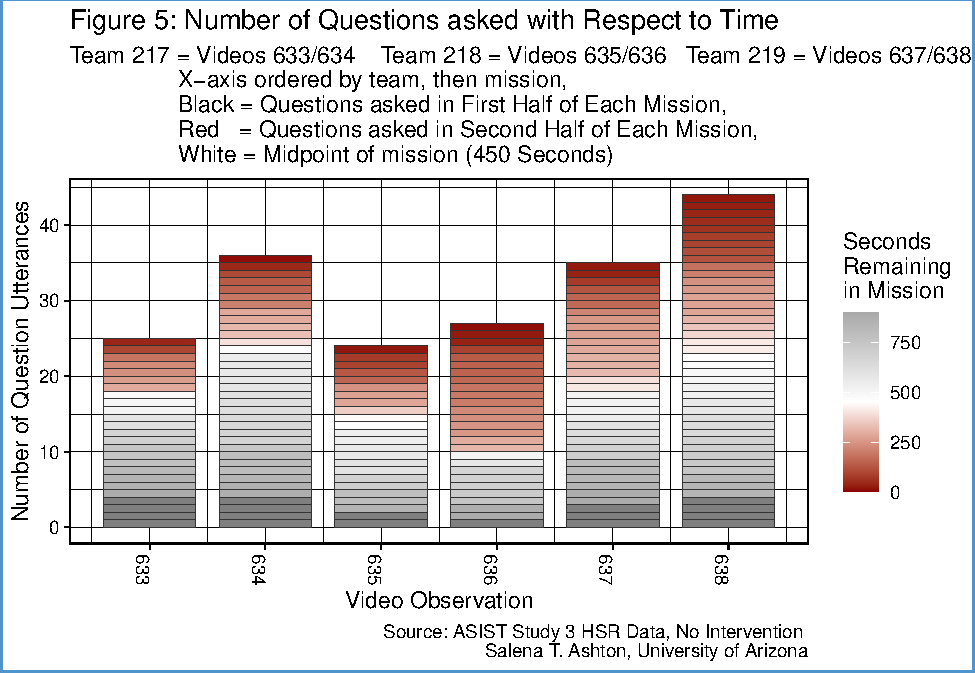
\includegraphics[width=0.9\textwidth]{../images/QuestionTiming_STA.pdf}}
    \caption{Questions asked with respect to time. Time is represented continuously as color within the histogram. Video observations and question count are represented as a histogram. Team 218 (videos 635 and 636) asked the fewest questions and scored the lowest combined point. Video 636 is colored red in more than 66\% of its bars, meaning that more than 66\% of questions were asked toward the end of the mission. Compare this to team 1 (videos 633 and 634), who were relatively quiet players and asked the most questions in the beginning of each mission. Team 3 asked the most questions. The even distribution of red and black demonstrates how they asked questions at a \emph{consistent rate} throughout their missions.}
    \end{figure}
    
%2 Figure 1 
\begin{figure}[h!]
    \centering
    \fbox{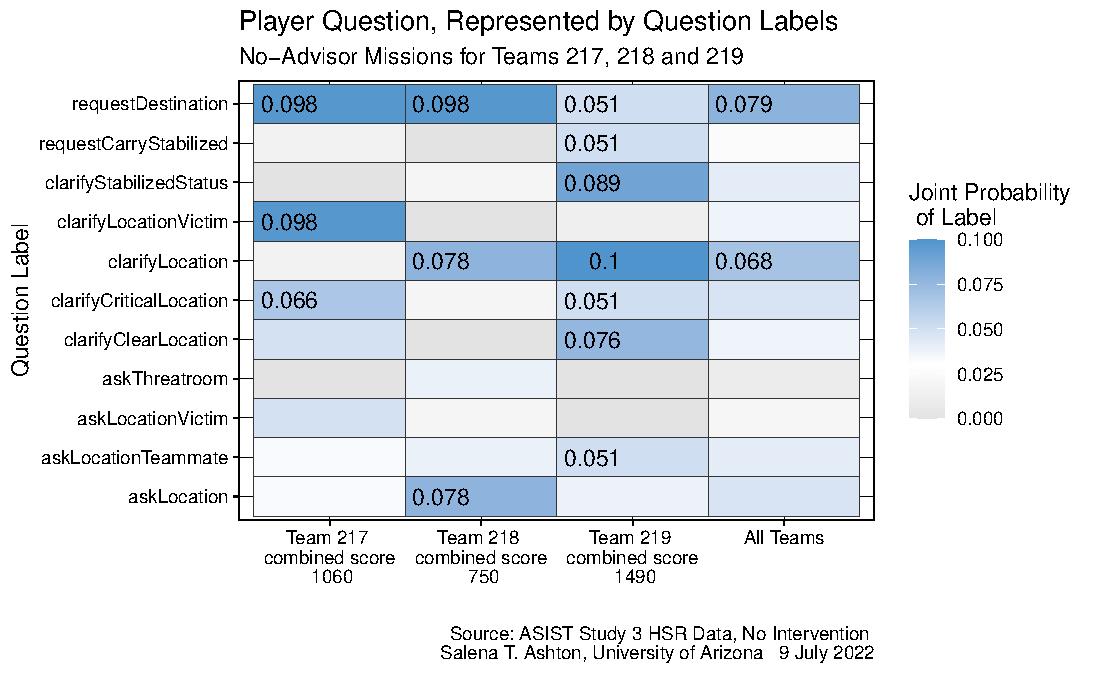
\includegraphics[width=0.9\textwidth]{../images/questionLabelProbability_STA.pdf}}
    \caption{Player question utterances, represented by question labels and displayed by each team and the most probable question labels. This shows the highest probability of questions to be asked: requests for teammates to come, clarification of a victim's status for transport, shown by the word 'stabilized' and not by 'victim' (an unstabilized victim), and clarification of any victim's location. Notice that team 219, who scored the highest of the three, asked more questions to clarify communication with each other. Previous assumptions about players who prioritized the clearing of rubble, navigation strategy or dividing up tasks is not supported in this preliminary investigation.}
\end{figure}

%3 Figure 2
\begin{figure}[h!]
    \centering
    \fbox{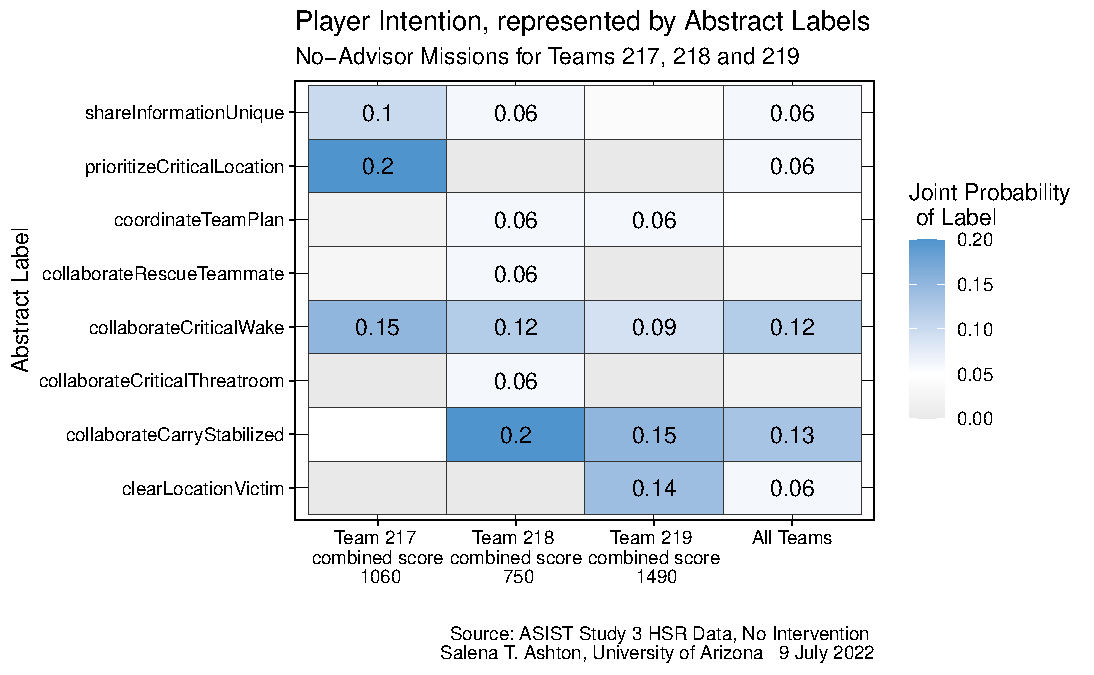
\includegraphics[width=0.9\textwidth]{../images/abstractLabelProbability_STA.pdf}}
    \caption{Player intention, represented by abstract labels and displayed by each team and the most probable abstract label. This shows the highest probability of intentions, expressed by questions, visual cues, context, and player interaction (represented as an abstract label). These include collaborating with teammates about waking critical victims and carrying stabilized victims to the proper sick bay. Team 219, who scored some of the highest combined scores in many of the observations, not just the ones annotated, compared to 218, who scored some of the lowest in the data, intended to collaborate on carrying stabilized victims to the proper sick bay. The difference in score is found in more granular actions: while team 219 often requested for collaborative tasks, team 218 would more often demand or tell others what tasks to perform (as seen in figure 1).}
\end{figure}

%4 Figure 3
\begin{figure}[h!]
    \centering
    \fbox{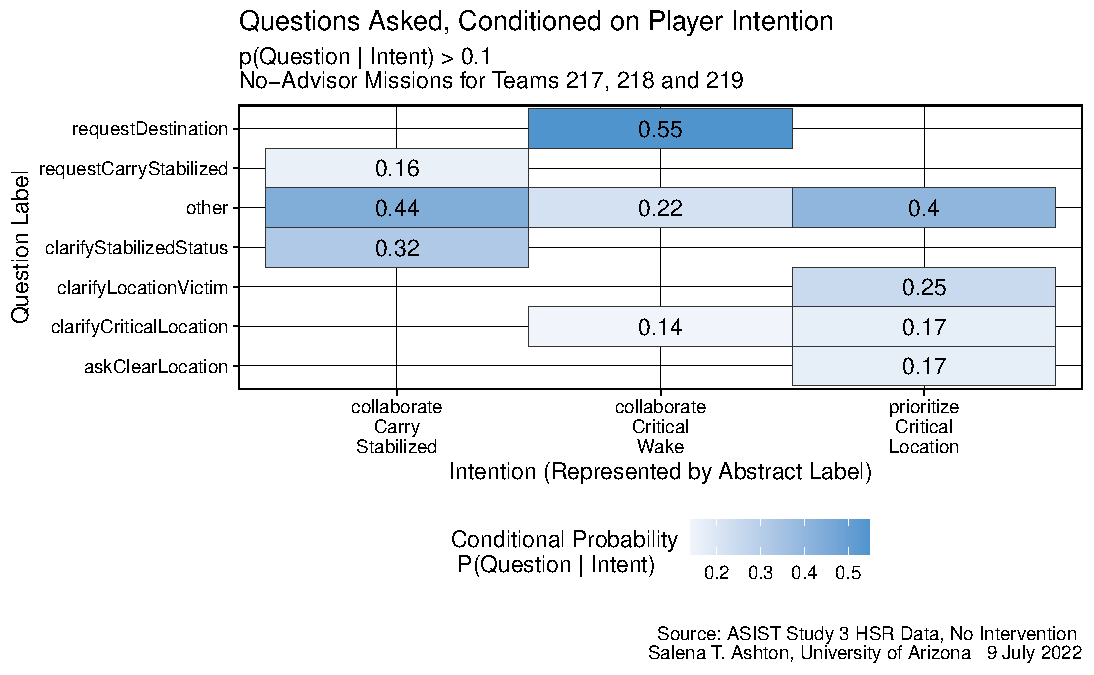
\includegraphics[width=0.9\textwidth]{../images/questionLabel_ConditionalProbability_STA.pdf}}
    \caption{Conditional probability of questions asked, given the player's intention. Variation of questions that can be asked, given player intention. More than 40\% of questions that could be asked are marked 'other,' (abstracted into 'other' category for clarity of this visual). It is this variation that matters: players will not necessarily ask expected questions (or any question at all) just because they have intention. The most likely questions that \emph{are vocalized} have one aspect in common: they all have verbs that are collaborative in nature: request, clarify, collaborate. Verbs that are less collaborative in nature, (direct, suggest, inform) do not show up as the most common questions. This suggests that when players feel like they are part of the team, they are more likely to ask questions that have a give-and-take dialog.}
\end{figure}

%5 Figure 4
\begin{figure}[h!]
    \centering
    \fbox{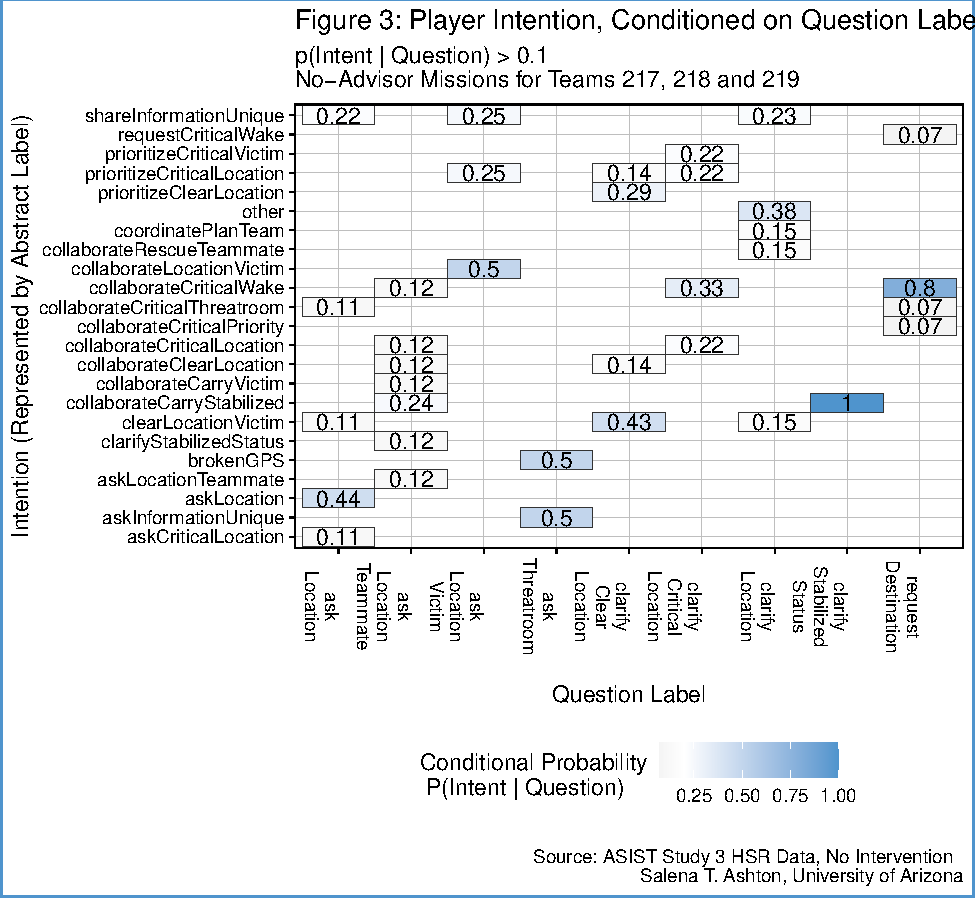
\includegraphics[width=0.9\textwidth]{../images/abstractLabel_ConditionalProbability_STA.pdf}}
    \caption{ Conditional probability of player intention, given the question that is asked. Players were most likely to ask for unique information from the engineer when they wanted to prioritize locations or learn about threat rooms. When the GPS systems failed, more than half of the time players asked about threat rooms, not victims, rubble, or other events. For example, the previous figure shows that when a player's intention is to wake a critical, they are 55\% likely to ask another player to join them (trivial). It is far more interesting to see in this figure that when the question utterance 'requestDestination', it is more than 80\% likely to be asked only for the intent of waking a critical victim.}
\end{figure}


    
%7 Figure 6
\begin{figure}[h!]
    \centering
    \fbox{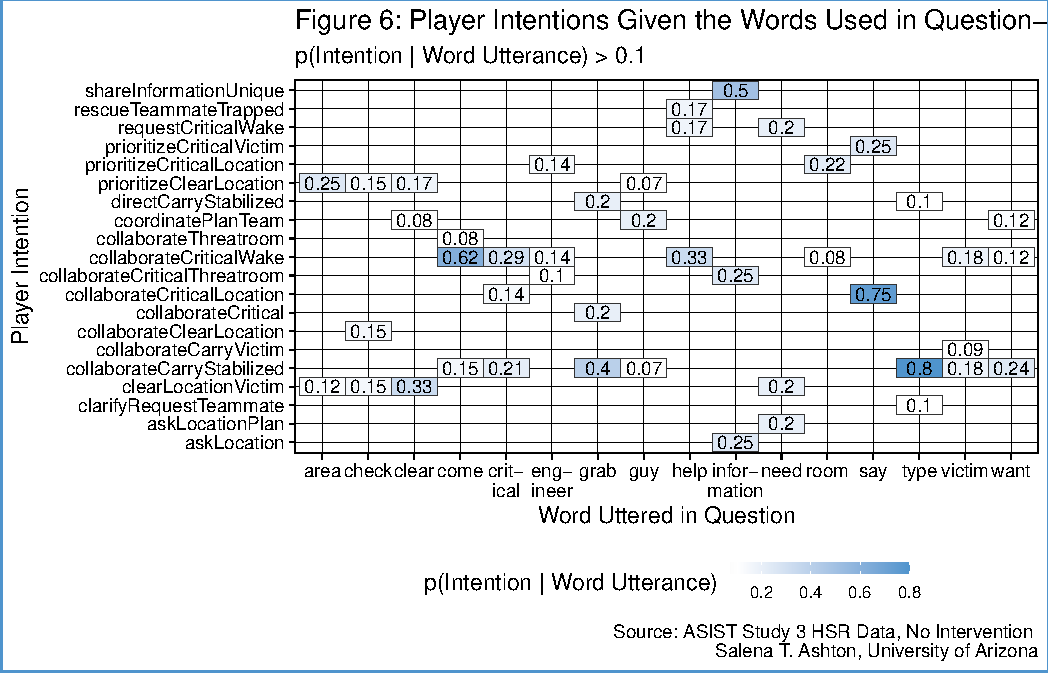
\includegraphics[width=0.9\textwidth]{../images/QuestionUtterances_Link_STA.pdf}}
    \caption{Conditional probabilities of player intention, given the words that a player speaks when asking a question. While some words can infer trivial player intention (ie. 'information' utterances show 'shareInformationUnique' intention), other words such as 'say', 'type', or 'come' are not domain-specific to the Minecraft environment-- yet show team collaboration about critical victims. 'Say' is the stemmed keyword that shows teammate communication and clarification (ie. \emph{"Did you say} ...") Compare this to words like 'critical' or 'area', which do not show team collaboration as much as it shows individual intention. }
    \end{figure}

%1 Figure 7
\begin{figure}[h!]
    \centering
    \fbox{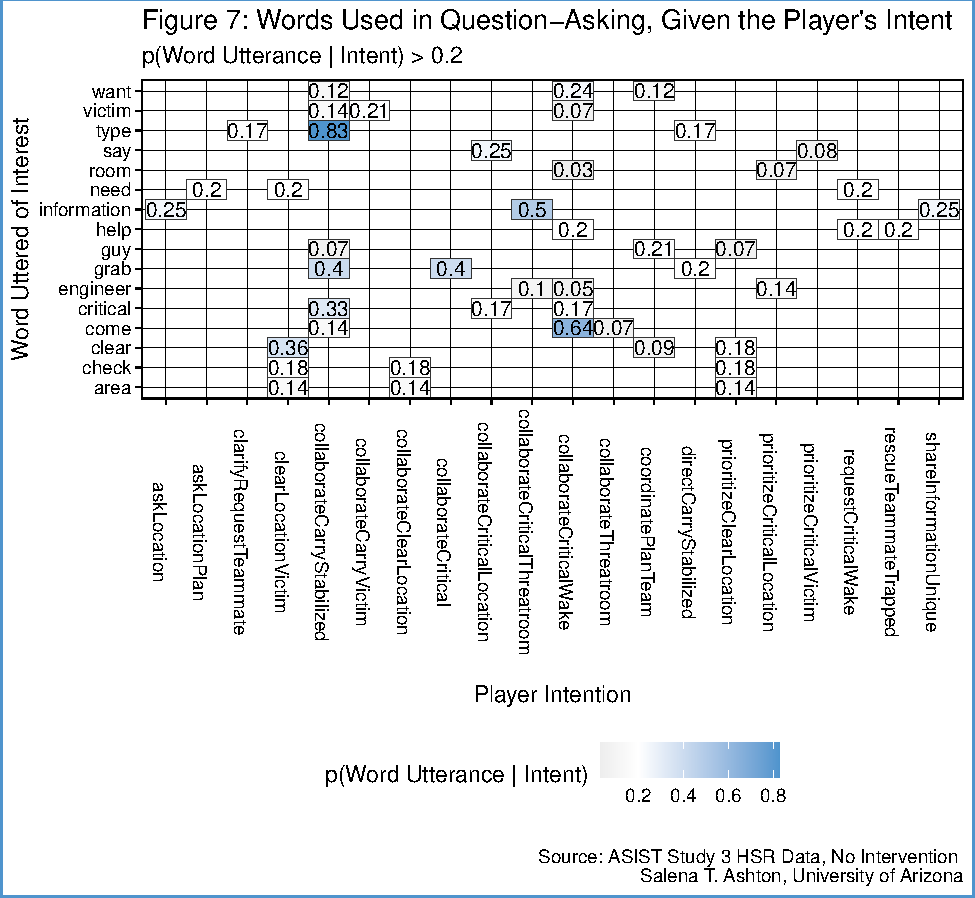
\includegraphics[width=0.9\textwidth]{"../images/Intent_to_Utterances_Link_STA.pdf"}}
    \caption{Conditional probabilities of words to be uttered in a question, given the player's intention. Returning to the intent of 'collaborateCriticalWake', the two most likely words to be uttered are 'want' and 'information.' From the previous figure, only the words 'come', 'critical', and 'help' tie back to this intent.}
    \end{figure}
 
    
     






